\documentclass[border=2pt]{standalone}
\usepackage[T1]{fontenc}
\usepackage{tikz}
\usepackage{amsmath,amssymb}
\usepackage{graphicx}
\usetikzlibrary{positioning, arrows.meta, fit, backgrounds, calc, decorations.pathreplacing}

% === Color palette ===
\definecolor{cBlue}{HTML}{3B7DD8}
\definecolor{cGreen}{HTML}{27AE60}
\definecolor{cPurple}{HTML}{8E44AD}
\definecolor{cGray}{HTML}{5D6D7E}

\begin{document}
\begin{tikzpicture}[
    >=Latex,
    block/.style={
        draw, rounded corners=2pt, minimum height=0.9cm,
        align=center, font=\small, line width=0.6pt
    },
    pb/.style={block, fill=cBlue!12, draw=cBlue!60},
    gb/.style={block, fill=cGray!10, draw=cGray!50},
    fb/.style={block, fill=cPurple!12, draw=cPurple!60},
    arr/.style={->, line width=0.7pt, draw=black!60},
    garr/.style={->, line width=0.7pt, draw=cGreen!70},
    shp/.style={font=\tiny\sffamily, text=black!55},
    fmap/.style={draw, line width=0.5pt, rounded corners=0.5pt},
]

% =============================================
% INPUT: stacked temporal satellite images
% =============================================

\def\imgsz{1.2cm}
\def\imgoff{0.2}

\foreach \i/\file in {3/input_dec, 2/input_sep, 1/input_jun, 0/input_mar} {
    \pgfmathsetmacro{\xoff}{\i * \imgoff}
    \pgfmathsetmacro{\yoff}{-\i * \imgoff}
    \node[inner sep=0pt, draw=black!40, line width=0.4pt] at ($(0.6 + \xoff, -0.6 + \yoff)$)
        {\includegraphics[width=\imgsz, height=\imgsz]{\file.png}};
}
\node[font=\tiny\sffamily, text=black!70] at (-0.35, -0.40) {Mar};
\node[font=\tiny\sffamily, text=black!70] at (-0.35, -0.60) {Jun};
\node[font=\tiny\sffamily, text=black!70] at (-0.35, -0.80) {Sep};
\node[font=\tiny\sffamily, text=black!70] at (-0.35, -1.00) {Dec};
\node[font=\footnotesize\sffamily, text=black!70] at (0.9, 0.4) {HLS Input};

% =============================================
% PRITHVI ViT BACKBONE
% =============================================

\node[pb, minimum width=2.0cm, minimum height=3.6cm] (vit) at (4.0, -0.65) {};
\node[font=\small, align=center] at (4.0, 0.65) {
    \textbf{Prithvi ViT}\\[-2pt]
    {\scriptsize encoder}
};

\node[pb, minimum width=1.5cm, minimum height=0.45cm, fill=cBlue!22] (blk5) at (4.0, 0.1) {
    {\scriptsize Layer 5}
};
\node[pb, minimum width=1.5cm, minimum height=0.45cm, fill=cBlue!22] (blk11) at (4.0, -0.45) {
    {\scriptsize Layer 11}
};
\node[pb, minimum width=1.5cm, minimum height=0.45cm, fill=cBlue!22] (blk17) at (4.0, -1.0) {
    {\scriptsize Layer 17}
};
\node[pb, minimum width=1.5cm, minimum height=0.45cm, fill=cBlue!22] (blk23) at (4.0, -1.55) {
    {\scriptsize Layer 23}
};

\node[font=\scriptsize, text=cBlue!50] at (4.0, -0.17) {$\vdots$};
\node[font=\scriptsize, text=cBlue!50] at (4.0, -0.73) {$\vdots$};
\node[font=\scriptsize, text=cBlue!50] at (4.0, -1.28) {$\vdots$};

\draw[arr] (1.85, -0.65) -- (vit.west);

% =============================================
% CONCAT MODULE (clean box)
% =============================================

% Vertical bus x-coordinate
\def\busx{5.6}

% Horizontal stubs from each layer to the bus (no arrowheads)
\draw[line width=0.7pt, draw=cGreen!70] (blk5.east)  -- (\busx, 0.1);
\draw[line width=0.7pt, draw=cGreen!70] (blk11.east) -- (\busx, -0.45);
\draw[line width=0.7pt, draw=cGreen!70] (blk17.east) -- (\busx, -1.0);
\draw[line width=0.7pt, draw=cGreen!70] (blk23.east) -- (\busx, -1.55);

% Vertical bus line connecting all stubs
\draw[line width=0.7pt, draw=cGreen!70] (\busx, 0.1) -- (\busx, -1.55);

% Single arrow from bus midpoint to concat
\node[fb, minimum width=1.8cm, minimum height=0.9cm] (concat) at (7.2, -0.65) {
    \textbf{Concat}
};

\draw[garr] (\busx, -0.65) -- (concat.west);

% =============================================
% 3D UPSCALER (single box)
% =============================================

\node[gb, minimum width=1.8cm, minimum height=0.9cm] (head) at (9.5, -0.65) {
    \textbf{3D}\\[-2pt]
    \textbf{Upscaler}
};

\draw[arr] (concat.east) -- (head.west);

% =============================================
% OUTPUT: 4 phenology DOY heatmaps (stacked vertically)
% =============================================

\def\outsz{0.9cm}
\def\outx{12.0}

% Greenup
\node[inner sep=0pt, draw=black!30, line width=0.4pt] (outG) at (\outx, 0.55)
    {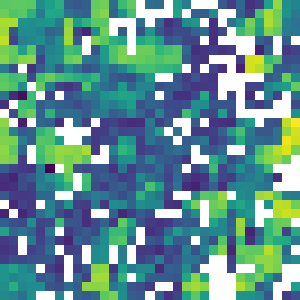
\includegraphics[width=\outsz, height=\outsz]{output_g.png}};
\node[font=\tiny\sffamily, text=black!60, right=2pt of outG] {G};

% Maturity
\node[inner sep=0pt, draw=black!30, line width=0.4pt] (outM) at (\outx, -0.55)
    {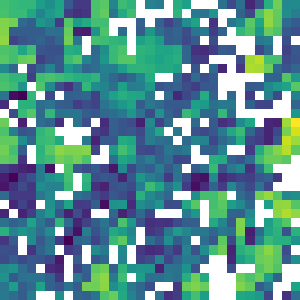
\includegraphics[width=\outsz, height=\outsz]{output_m.png}};
\node[font=\tiny\sffamily, text=black!60, right=2pt of outM] {M};

% Senescence
\node[inner sep=0pt, draw=black!30, line width=0.4pt] (outS) at (\outx, -1.65)
    {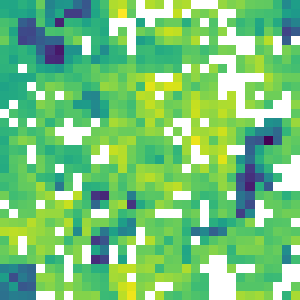
\includegraphics[width=\outsz, height=\outsz]{output_s.png}};
\node[font=\tiny\sffamily, text=black!60, right=2pt of outS] {S};

% Dormancy
\node[inner sep=0pt, draw=black!30, line width=0.4pt] (outD) at (\outx, -2.75)
    {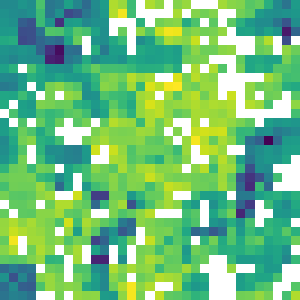
\includegraphics[width=\outsz, height=\outsz]{output_d.png}};
\node[font=\tiny\sffamily, text=black!60, right=2pt of outD] {D};

\node[font=\footnotesize\sffamily, text=black!70] at (\outx, 1.25) {DOY Predictions};

% Branching arrows from 3D Upscaler to outputs
\coordinate (outsplit) at (11.0, -0.65);
\draw[arr] (head.east) -- (outsplit);
\draw[arr] (outsplit) |- (outG.west);
\draw[arr] (outsplit) |- (outM.west);
\draw[arr] (outsplit) |- (outS.west);
\draw[arr] (outsplit) |- (outD.west);

% =============================================
% BACKGROUND SHADING
% =============================================

\begin{scope}[on background layer]
    \node[
        fill=cBlue!5, rounded corners=6pt, inner sep=6pt,
        fit=(vit),
        label={[font=\scriptsize\sffamily, text=cBlue!60]above:{\itshape Pretrained}}
    ] {};
    \node[
        fill=cPurple!5, rounded corners=6pt, inner sep=6pt,
        fit=(concat),
        label={[font=\scriptsize\sffamily, text=cPurple!50]above:{\itshape Learned}}
    ] {};
\end{scope}

\end{tikzpicture}
\end{document}
